\section{High-level Overview}

%% General introduction about the SchIM
In this section, we provide a high-level description of the
organization of the proposed scheduler in-the-middle. As previously
mentioned, the \schim leverages the PLIM approach originally proposed
in~\cite{PLIM20}. Indeed, CPU-originated main memory transactions are
re-routed through the programmable logic and scheduled by the \schim
according to a flexible and configurable policy. The result is that
the timing of memory transactions generated by real-time applications
can be carefully determined and reasoned upon. 

Because the \schim follows a PLIM approach, transactions can be
selectively sent to the \schim for scheduling. It is always possible,
however, to dynamically exclude the \schim and instead route
transactions directly to main memory. For the purpose of this paper,
however, we mainly consider a setup in which all the CPU-generated
memory transactions are handled by the \schim.

Figure~\ref{fig:block_diagram} provides an overview of the location of
the \schim within the main components of the target platform. The
highlighted {\bf COLOR} path depicts the route that memory requests
originated by the CPUs follow when the SchIM is used. Application
memory requests can reach the \schim through multiple
interfaces. Without loss of generality, we consider a \schim instance
with two arrival lanes, which are labeled as \axiin{1} and \axiin{2}
in Figure~\ref{fig:block_diagram}. The \schim then forwards the
received transactions towards main memory through the \axiout{3}
interface. A more detailed view of the \schim module is provided in
Figure~\ref{fig:MemorEDF_module_schema} where the same convention is
used to identify input and output ports. In addition, as shown in
Figure~\ref{fig:MemorEDF_module_schema}, a fourth \axiconf{4} port is
used to configure the \schim module from the PS.

%% The objective of the module is to arbitrate the access of the bus to
%% the main memory between the different cores of the PS side at the
%% transaction level by enforcing a given policy.  Roughly, the module
%% receives transactions from the PS side, acknowledges them and finally
%% repeat them with the main memory as destination.  The exact order in
%% which inter-core transactions are being repeated is decided by an
%% embedded on-chip hardware scheduler.

\begin{figure}
  \centering
  \begin{tikzpicture}[scale=0.6, every node/.style={scale=0.6}]
    % Modules
    \draw[fill={rgb:black,1;white,7}] ( 0.0, 0.0) rectangle ( 4.0, 4.0) node[pos=.5] {PS};
    \draw[fill={rgb:black,1;white,7}] ( 6.0, 0.5) rectangle ( 8.0, 2.5) node[pos=.5] {SchIM};
    \draw[fill={rgb:black,1;white,7}] (10.0, 0.5) rectangle (12.0, 2.5) node[pos=.5] {Bleacher};
    % Outline PL
    \draw[dashed] ( 0.0, 4.0) -- ( 4.0, 4.0) -- ( 4.0, 0.0) -- (14.0, 0.0) -- (14.0, 6.0) -- ( 0.0, 6.0) -- ( 0.0, 4.0);
    % Buses
    % PS to SchIM HPM0
    \draw[{Stealth}-{Stealth}] ( 4.0, 1.5) -- ( 6.0, 1.5) node[above, pos=.5] {Transactions};
    % SchIM to Bleacher HPM0
    \draw[{Stealth}-{Stealth}] ( 8.0, 1.5) -- (10.0, 1.5) node[above, pos=.5] {Transactions};
    % SchIM to Bleacher HPM0
    \draw[{Stealth}-{Stealth}] (12.0, 1.5) -- (13.0, 1.5) -- (13.0, 5.0) -- ( 2.0, 5.0) node[above, pos=.5] {Transactions} -- ( 2.0, 4.0);
    % PS to SchIM and Bleacher LPD
    \draw[{Stealth}-{Stealth}] ( 4.0, 3.0) -- (11.0, 3.0) node[above, pos=.5] {Configuration} -- (11.0, 2.5);
    \draw[-{Stealth}] ( 7.0, 3.0) -- ( 7.0, 2.5);
\end{tikzpicture}

  \caption{High-level block design of the proposed \schim
    module. \emph{RM: we need to replace this picture with one that
      provides more details about the main blocks of the platforms. We
      also do not need to include the bleacher as it is not
      fundamental for the operation of the \schim.}}
  \label{fig:SchIM_overview_schema}
\end{figure}


%% Micro-architecture and first list of modules

\subsection{Micro-architecture}
\label{subsec:micro-arch}

The \schim module is composed of a number of sub-modules grouped into
three different domains, namely (i) the \emph{interfacing domain},
(ii) the \emph{queuing domain}, and (iii) the \emph{scheduling
  domain}.

The interfacing domain encompasses the sub-modules in charge of
interfacing the core logic of the \schim with the rest of the system
using the AXI protocol.  This domain is comprised of three
sub-modules. These are (i) the \emph{packetizer}, (ii) the
\emph{serializer}, and (iii) the previously mentioned configuration
interface.

The PS-facing end of the {\bf packetizer} offers an AXI slave port to
accept new incoming transactions. Upon receipt, this module transforms
each transaction into an equivalent \emph{packet} that can be queued
and scheduled by the rest of the \schim. Packetization of AXI
transactions is necessary to be able to store transactions that are
serial by nature.  Indeed, a standard AXI transaction is composed of
one address phase (AR or AW channel) followed by a data phase (R or W
channel) which can be itself composed of multiple successive bursts.

In many ways, the {\bf serializer} is the dual module of the
packetizer. Its purpose is to transform the packets that encode
CPU-generated memory requests back into AXI-compliant transactions. As
such, the serializer offers a master port to the rest of the system to
be routed to the main memory controller.

%% purpose of slave and master ports, they are also in charge of
%% respectively transforming the AXI transactions into an equivalent
%% packet and to transform these packets 

The queuing domain is in charge of the storing the incoming
transactions emitted by the PS side.  The motivation behind the use of
queues is implied by the fact that all the masters located on the PS
side share a common AXI bus (namely HPM0 as shown in figure
\ref{fig:SchIM_overview_schema}).  Therefore, in order to cancel the
Round Robin arbitration policy applied in the PS side and in order to
avoid that one high priority core is stalled by a lower priority one,
each core is granted a queue within the \schim module.  Not only the
queues act as containers and buffers for transactions, they also embed
logic and provide information to the scheduling domain regarding their
current state in order to avoid the queues to overflow or underflow
similarly to the producer-consumer problem.  As suggested by figure
\ref{fig:MemorEDF_module_schema}, transactions are inserted to the
adequate queues on the basis of the emitters identifier via the
dispatcher module.  Similarly, transactions are evicted from their
queue, routed by the selector module and sent directly to the output
of the module upon the action of the scheduling domain.

The scheduling domain encompasses all the sub-modules that enable
arbitration of the bus between the transactions issued by the
different cores of the PS side. Hence, this domain boasts several
transaction schedulers implemented at the hardware level.  The
scheduling policies offered by \schim include Fixed Priority (FP), Time
Division Multiple Access (TDMA), Earliest Deadline First (EDF), Least
Laxity First (LLF) and MemGuard (MG).  Each of the parameters required
by the aforementioned algorithms such as the priorities, the periods,
the deadlines and the budgets are re-configurable at the run-time
thanks to the inclusion of a configuration port.  Finally, the
scheduling domain is also the one in charge of the control of the
remaining the \schim module, driving and selecting the adequate signals
and ensuring the coherence and integrity of the data.

\begin{figure}
  \centering
  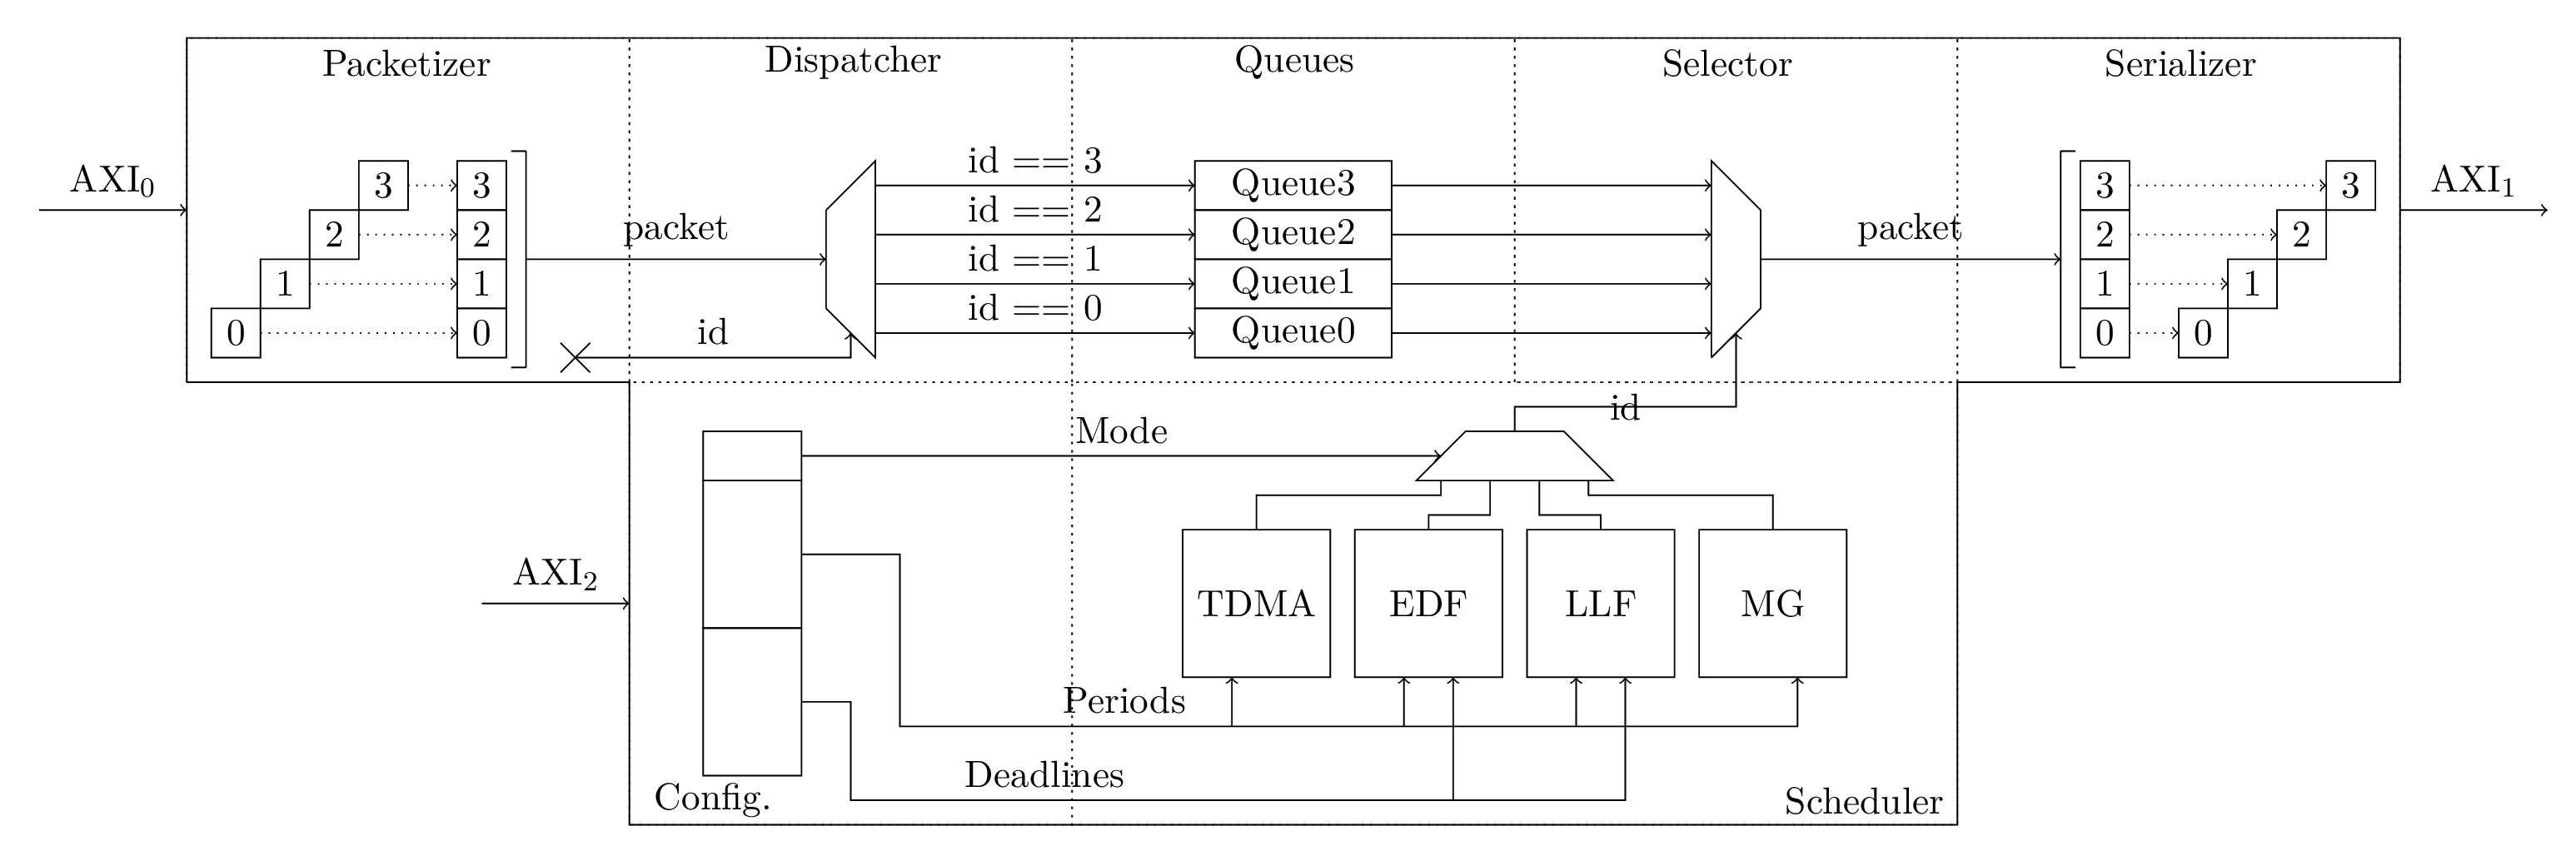
\includegraphics[scale=0.08]{images/MemorEDF_module_schema.png}
  \caption{Caption}
  \label{fig:MemorEDF_module_schema}
\end{figure}

\subsection{Modules Overview}

\par{\bf Packetizer:} The packetizer module transforms transactions on
the asynchronous AXI bus into schedulable entities to be queued at any
of the \schim queues.

\subsection{Transactions Life Cycle}
\label{subsec:transaction-life-cycle}

Let us consider a system with four cores (noted $C = \{c_{0}, c_{1},
c_{2}, c_{3}\}$) sending transactions $T = \{t_{0}, t_{1}, ...,
t_{n}\}$ to the \schim module.  Consequently, the latter boasts four
queues (noted $Q = \{q_{0}, q_{1}, q_{2}, q_{3}\}$) buffering the
transactions under the form of packets $P = \{p_{0}, p_{1}, ...,
p_{n}\}$ where $p_{i} = Packetizer(t_{i})~\forall i \in [0 : n]$.

In the present example, we will assume $t_{1}$ as being the
transaction under analysis.  The latter is emitted by $c_{2}$ in
direction of the \schim module.  The packetizer receives this
transaction and, once the AXI protocol completed, transform it into an
equivalent packet $p_{1} = Packetizer(t_{1})$.  Following this
transformation, the newly created packet is forwarded to the
dispatcher which, thanks to the emitter's id embedded within the
transaction, is re-routed to the corresponding queue $q_{2}$ (since
emitted by $c_{2}$).  After the insertion of $p_{1}$ in $q_{2}$, the
state of the queuing domain is as follows: $q_{0}$ has two packets
$p_{0}$ and $p_{k}$ and $q_{2}$ only has $p_{1}$.  At this point,
$q_{0}$ is considered for scheduling by the scheduling domain.  In
consequence, $p_{0}$ is forwarded to the serializer through the
selector.  Simultaneously to the reception of the packet by the
serializer, the latter receives an activation signal from the
scheduling domain informing the serializer that the packet is valid
and that a transaction can be started.  Similarly to the packetizer,
the serializer will transform the packet $p_{0}$ back to its initial
AXI transaction form $t_{0} = Serializer(p_{0})$.  Thereafter, once
the $t_{0}$ has been sent, the serializer will inform the scheduling
domain via a signal, that he is ready to accept the next packet as
input.  Upon the reception of this signal, the scheduling domain will
both re-direct the latter to the queue of the previous packet to
indicate that it has been consumed and change the selected queue
according to the scheduling policy so that the first packet of this
queue can be forwarded to the serializer through the selector module.
In the present example, the "consumed" signal forwarded by the
scheduler is sent to $q_{0}$ which is then empty.  At this instant,
two scenarios are possible:

\begin{enumerate}
\item $q_{0}$ is still considered for scheduling following the
  selected scheduling policy. Therefore, as $q_{0}$ is empty, it
  outputs an "empty" signal received by the scheduling domain.  The
  latter then decides to not send any activation signal to the
  serializer because there is nothing left to transmit in the selected
  queue.  In other words, the access to the main memory is being
  stalled on purpose by the scheduling policy i.e. the scheduling
  policy is not work conserving.  For instance, such a scenario could
  happen in the case of TDMA or if all the queues are empty.  The
  logic will resume as soon as the selected queue is filled.
\item $q_{2}$ is now considered instead of $q_{0}$ for scheduling.  In
  this case, the "consumed" signal is repeated to $q_{0}$ while the
  queue ID changes in order to select $q_{2}$.  This results in the
  packet contained inside $q_{1}$ to be forwarded to the selector.
\end{enumerate}

